\documentclass{ctexart}
\usepackage{amsmath}
\usepackage{geometry}
\usepackage{graphicx}
\usepackage{booktabs}
\usepackage{hyperref}
\usepackage{float}
\title{光源的时间相干性}
\author{陈启钰\,\,2300011447}
\date{\today}
\begin{document}
	\maketitle
	\section{白光的相干长度和相干时间}
	实验测量得到等厚干涉条纹左右对称时,$M_1$位置
	\begin{align}
		d_0=51.132\mathrm{mm}
	\end{align}
	测量得到级次
	\begin{align}
		k_1=2
	\end{align}
	相干长度
	\begin{align}
		\Delta L_1=1.1\times10^{-6}\mathrm{m}
	\end{align}
	相干时间
	\begin{align}
		\Delta t_1=\frac{\Delta L_1}{c}=3.7\times 10^{-15}\mathrm{s}
	\end{align}
	\section{通过橙色玻璃}
	级次
	\begin{align}
		k_2=11
	\end{align}
	相干长度、时间为
	\begin{align}
		\Delta L_2=6.9\times10^{-6}\mathrm{m},\Delta t_2=2.3\times10^{-14}\mathrm{s}
	\end{align}
	\section{通过黄干涉滤光片}
	级次
	\begin{align}
		k_3=62
	\end{align}
	相干长度、时间为
	\begin{align}
		\Delta L_3=3.6\times10^{-5}\mathrm{m},\Delta t_3=1.2\times10^{-13}\mathrm{s}
	\end{align}
	\section{测量汞双黄线的波长差}
	\subsection{采用拍测量}
	实验测得各个可见度为零的点的坐标列表如下。
	\begin{table}[H]
		\begin{center}
			\begin{tabular}{c|ccccccc}
				$i$&1&2&3&4&5&6&7\\\hline
				$d_i/\mathrm{mm}$&51.497&51.418&51.334&51.253&51.174&51.103&51.021\\				
			\end{tabular}
		\end{center}
	\end{table}
	采用最小二乘法拟合,得到
	\begin{align}
		\Delta d=0.0792\mathrm{mm},r=0.9998
	\end{align}
	可计算波长差
	\begin{align}
		\Delta \lambda_1=\frac{\bar{\lambda}}{2\Delta d}=2.11\mathrm{nm}
	\end{align}
	\subsection{通过光电记录的光强数据计算}
	计数得到一个拍内光强峰有$\Delta k=272$个,于是
	\begin{align}
		\Delta \lambda_2=\frac{\bar{\lambda}}{\Delta k}=2.13\mathrm{nm}
	\end{align}
	可见,两种方法测量得到的结果十分相近。
	\section{原始数据}
	\begin{figure}[H]
		\centering
		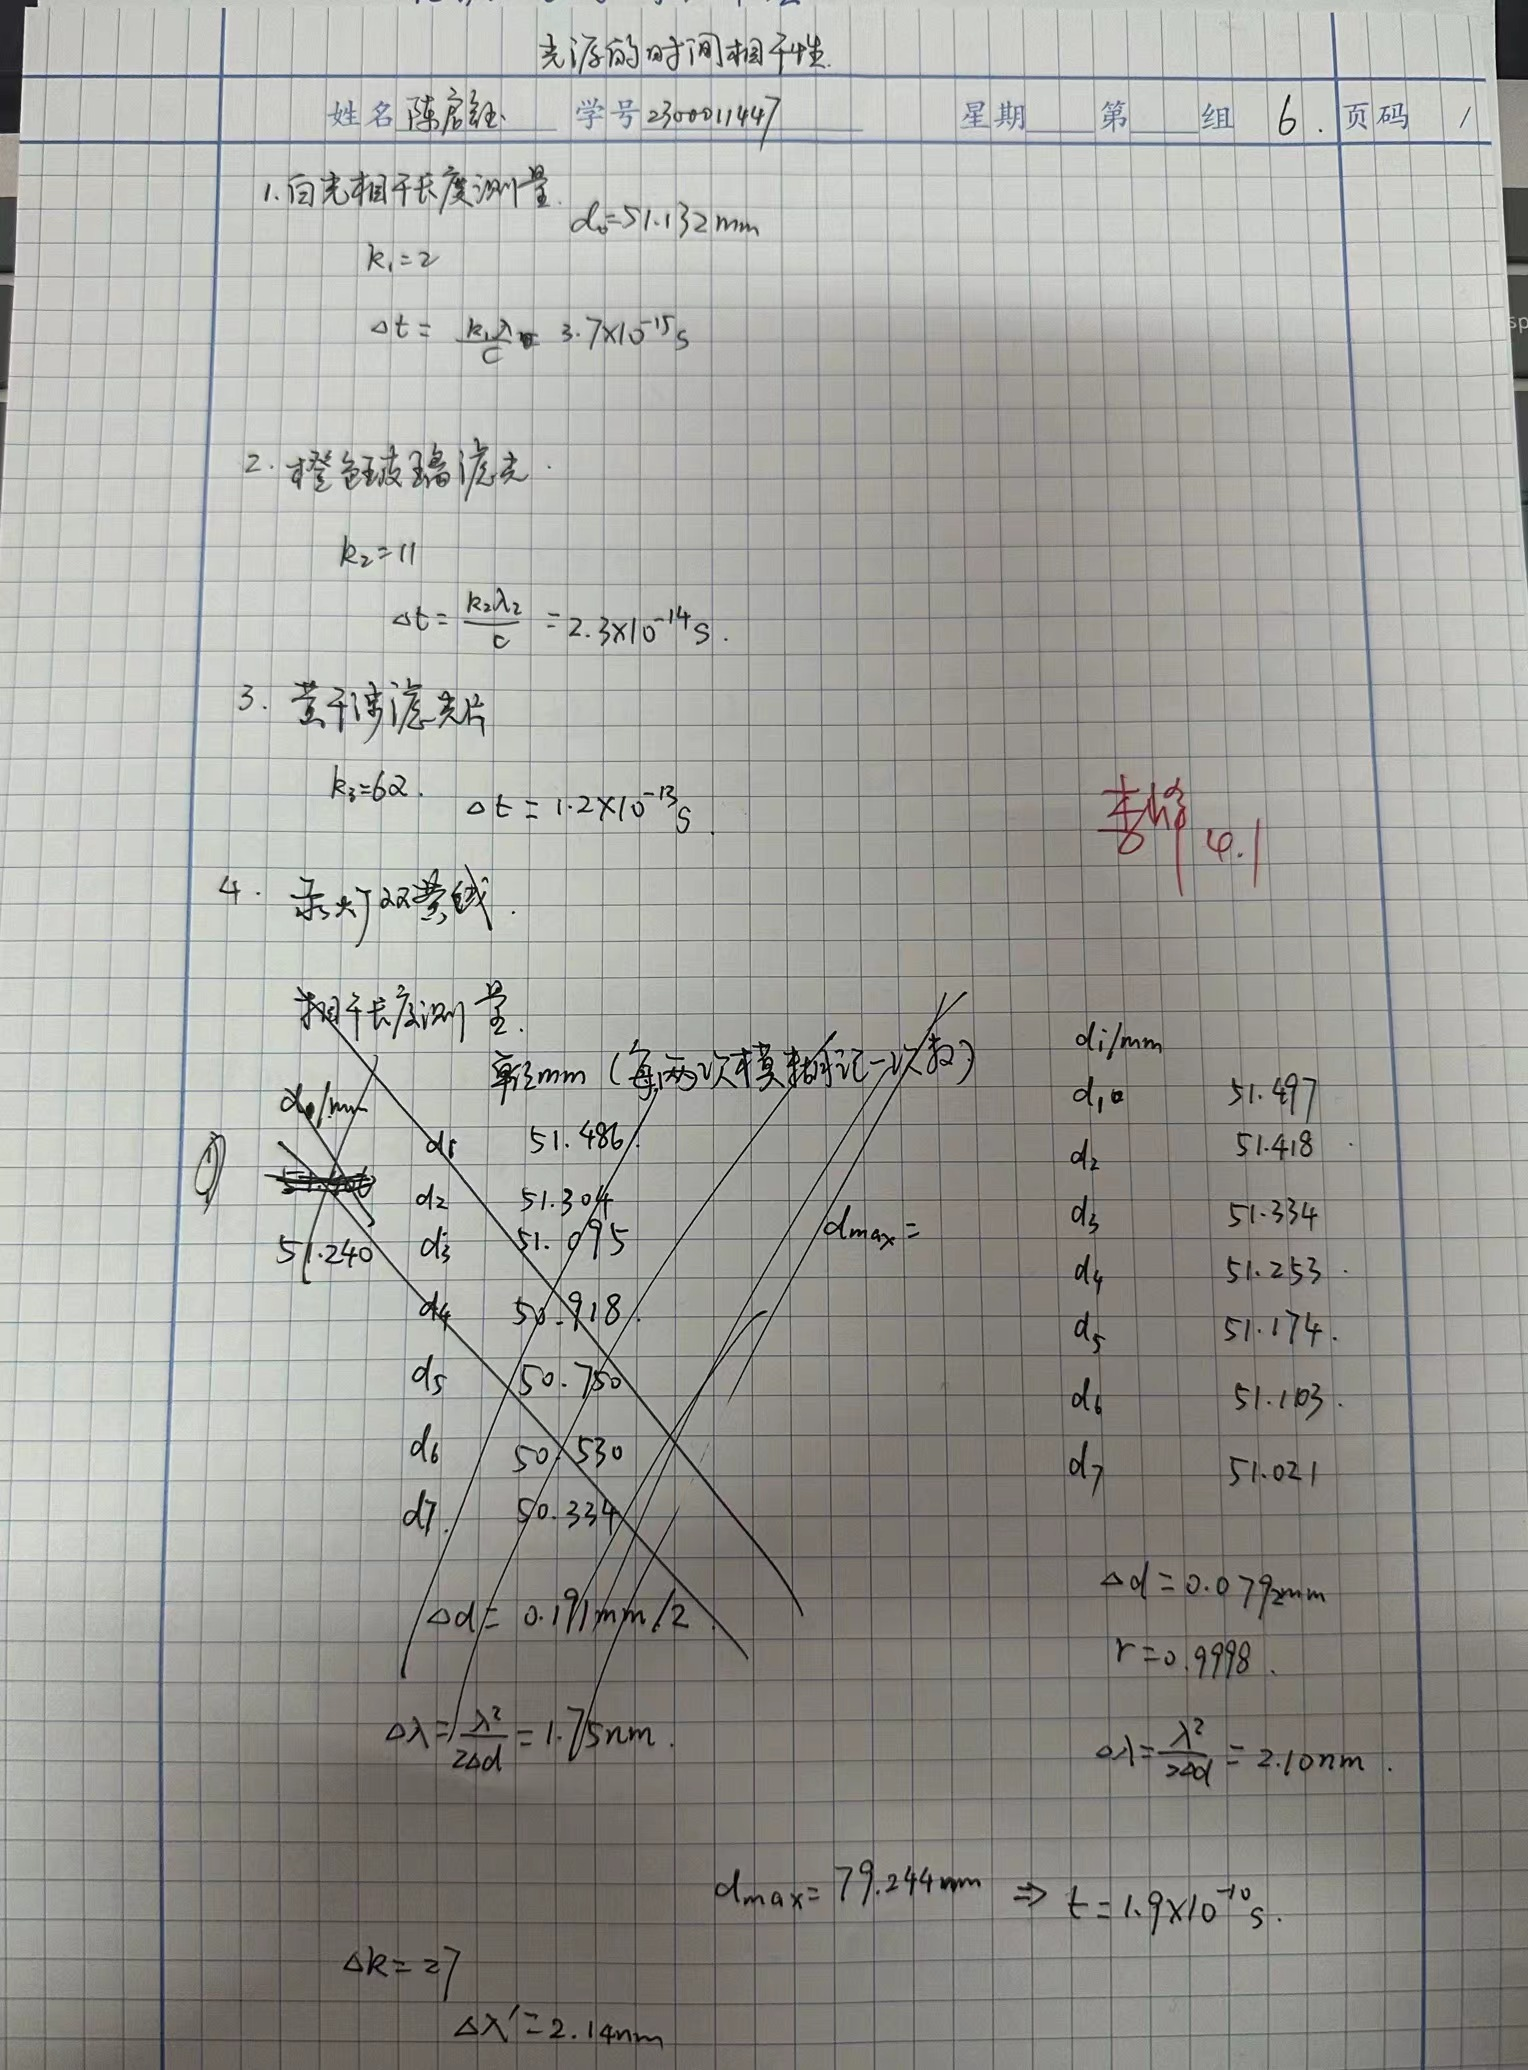
\includegraphics[width=14cm]{fig.jpg}
	\end{figure}
\end{document}